\documentclass{article}
\usepackage[utf8]{inputenc}
\usepackage{amsmath}
\usepackage{flexisym}
\usepackage{graphicx}
\graphicspath{ {./images/} }
\usepackage[]{algorithm2e}
\usepackage[font=small,labelfont=bf]{caption} % Required for specifying captions to tables and figures
\usepackage{url}
\usepackage{enumitem}
\usepackage{listings}
\title{DV2574 - Assignment 3}
\author{Niklas Br�nnlund}
\date{March 2019}

\begin{document}
\maketitle

\section*{Problems}
    \section{Recurrent neural network (RNN)}

    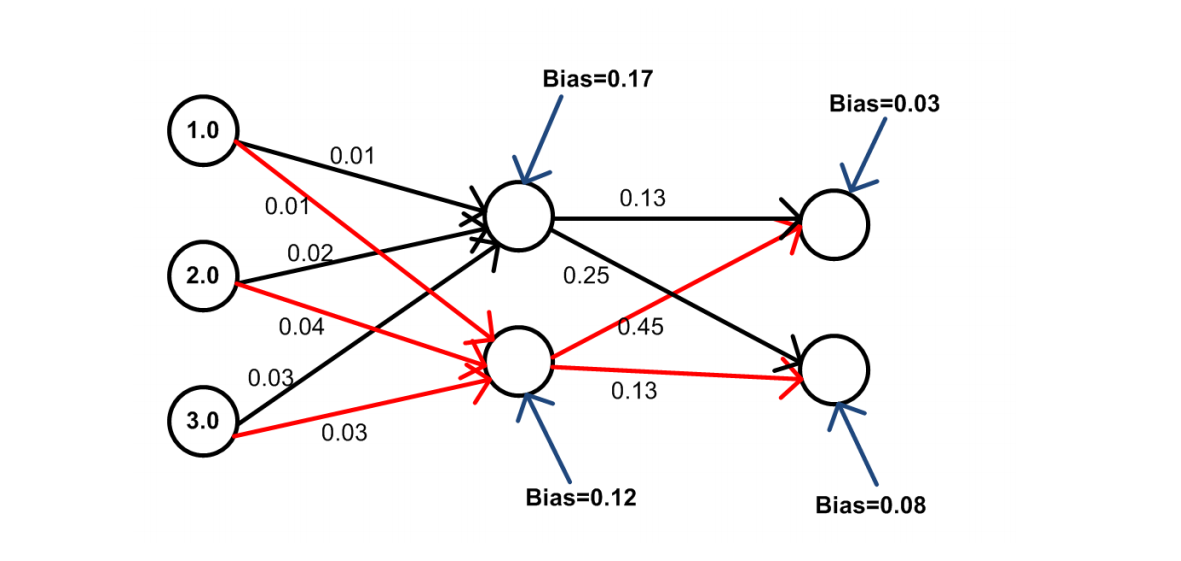
\includegraphics[width=\textwidth]{nn}
    Given the recurrent neural network above, we can conclude that it has the following properties:
    \begin{enumerate}[label=(\alph*)]
        \item 14 weights and biases
        \item 6 input-to-hidden weights
        \item 2 hidden node biases
        \item 4 hidden-to-output weights
        \item 2 output nodes 
        \item The input values of the network is 1,2,3
        \item Hidden node 1: $1*0.01 + 2*0.02 + 3*0.03 + 0.17 = 0.31 => \tanh(0.31)$, Hidden node 2: $1*0.01 + 2*0.04 + 3*0.03 + 0.12 = 0.3 => \tanh(0.3)$\\ Output node 1: $y_1 = \tanh(0.31) * 0.13 + \tanh(0.3)*0.45 + 0.03 = 0.200147$\\
        Output node 2: $y_2 = \tanh(0.31)*0.25 + \tanh(0.3)*0.13 + 0.08 = 0.192980$.\\ By using the Softmax function
        \begin{equation}
            S(y_i) = \frac{e^{y_i}}{\sum_j e^{y_j}}
        \end{equation}
        \begin{equation}
            S(y_1) = \frac{\exp{0.200147}}{\exp{0.200147} + \exp{0.192980}}
        \end{equation}
        \begin{equation}
            S(y_2) = \frac{\exp{0.192980}}{\exp{0.200147} + \exp{0.192980}}
        \end{equation}
        \item The values of the hidden nodes will be stored in two context nodes which sits below the hidden nodes. These will act as supplementary input for the hidden nodes in the next iteration  
    \end{enumerate}
    
    \section{Convolutional neural network (CNN)}
    \subsection{Question $\textbf{a}$}
    Given an input image size of 416x416x1 and the following information
    
    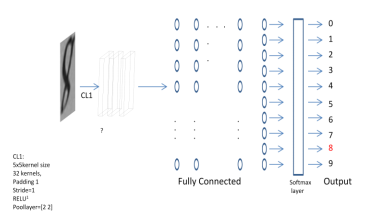
\includegraphics[width=\textwidth]{image1}
    \captionof{figure}{Figure of one convolutional layer}
    we can find the number of inputs for the fully connected neural network by going through the layers 
    \begin{enumerate}
        \item Convolutional
        \item Rectifier Linear Unit
        \item Pool
    \end{enumerate}

    The output from the Convolutional layer is calculated with
    \begin{equation}
        O = \frac{(W - K + 2P)}{S} + 1
    \end{equation}
    where W is the width of the input image, K is the 1D-kernel size, P is the padding and S is the strid. Given the convolutional layer in Figure 1, we have the following values W = 416, K = 5, S = 1, P = 1 and we use 32 filters. This will produce the output value
    \begin{equation}
        O = \frac{(416 - 5 + 2)}{1} + 1 = 414
    \end{equation}
    So in this case, after we apply one filter the output size will be 414x414. When we apply 32 filters we have the output size of 414x414x32. After applying the Rectifiera Linear Unit and Pool layer we have the output size 207x207x32. This will mean that we will have 
    \begin{equation}
    207x207x32 = 1371168 
    \end{equation}
    number of inputs for the fully connected neural network
    \subsection{Question b}
    In this question we have an input image of size 128x128x1 and we have the following setup of layers\\
    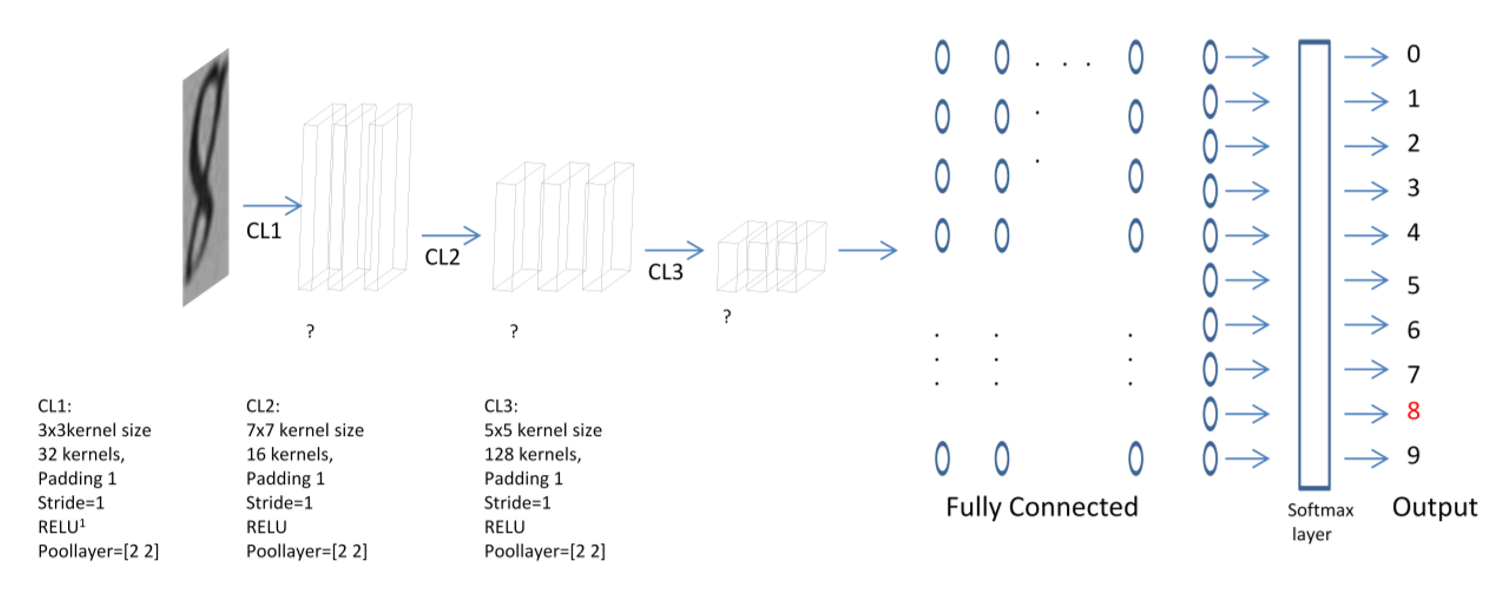
\includegraphics[width=\textwidth]{image2}
    \captionof{figure}{Figure of three convolutional layer}
    We will apply three different convolutional layers and if we use the same procedure as described previously we will start by calculating the output from the first convolutional layer. In the first layer we have the following variables:
    W = 128, K = 3, S = 1, P = 1 and we have 32 filters. This will produce an output of
    \begin{equation}
        O = \frac{(12 - 3 + 2)}{1} + 1 = 128
    \end{equation}
    which will produce an output size of 128x128x32 since we apply 32 filters. After applying Rectifier linear unit and pooling layer we get 62x62x32. This produces the following values for the second convolutional layer:
    W = 64, K = 7, S = 1, P = 1 and we have 16 filters. Given this we get an output of
    \begin{equation}
        O = \frac{(64 - 7 + 2)}{1} + 1 = 60
    \end{equation}
    for the second convolutional layer. Since we have 16 filters, the output size will be 60x60x16 and after rectifier linear unit and pool layer we get 30x30x16. The last convolutional layer will then have the values:
    W = 30, K = 5, S = 1, P = 1 and 128 filter which will produce output
    \begin{equation}
        O = \frac{(30 - 5 +2)}{1} + 1 = 28
    \end{equation}
    which, with 128 filters, will produce an output size of 28x28x128. And after rectifiera linear unit and pool layer we get 14x14x128. This means that the number of inputs for the fully connected neural network will be
    \begin{equation}
        14x14x128 = 25088
    \end{equation}
    
\end{document}
